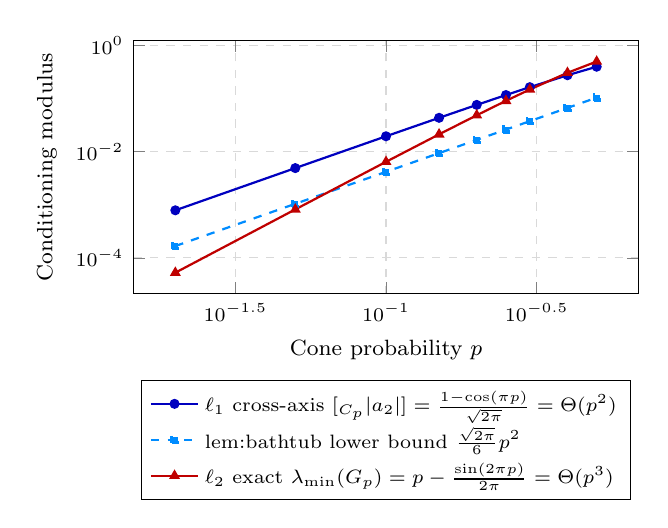
\begin{tikzpicture}
  \begin{loglogaxis}[
    width=0.66\textwidth,
    height=4.8cm,
    xlabel={Cone probability $p$},
    ylabel={Conditioning modulus},
    grid=major,
    grid style={dashed,gray!30},
    tick label style={font=\scriptsize},
    label style={font=\footnotesize},
    legend style={at={(0.5,-0.34)}, anchor=north, legend columns=1, font=\scriptsize, cells={anchor=west}}
  ]
    \addplot[blue!75!black, thick, mark=*, mark size=1.4pt] coordinates {
      (0.02, 7.872e-4) (0.05, 4.912e-3) (0.10, 1.953e-2) (0.15, 4.348e-2)
      (0.20, 7.619e-2) (0.25, 1.168e-1) (0.30, 1.644e-1) (0.40, 2.757e-1) (0.50, 3.989e-1)
    };
    \addlegendentry{$\ell_1$ cross-axis $\E[\ind_{C_p}|a_2|] = \frac{1-\cos(\pi p)}{\sqrt{2\pi}} = \Theta(p^2)$}
    \addplot[blue!45!cyan, dashed, thick, mark=square*, mark size=1.1pt] coordinates {
      (0.02, 1.671e-4) (0.05, 1.044e-3) (0.10, 4.178e-3) (0.15, 9.400e-3)
      (0.20, 1.671e-2) (0.25, 2.611e-2) (0.30, 3.760e-2) (0.40, 6.684e-2) (0.50, 1.044e-1)
    };
    \addlegendentry{\cref{lem:bathtub} lower bound $\frac{\sqrt{2\pi}}{6}p^2$}
    \addplot[red!75!black, thick, mark=triangle*, mark size=1.5pt] coordinates {
      (0.02, 5.260e-5) (0.05, 8.184e-4) (0.10, 6.451e-3) (0.15, 2.124e-2)
      (0.20, 4.863e-2) (0.25, 9.085e-2) (0.30, 1.486e-1) (0.40, 3.065e-1) (0.50, 5.000e-1)
    };
    \addlegendentry{$\ell_2$ exact $\lambda_{\min}(G_p) = p - \frac{\sin(2\pi p)}{2\pi} = \Theta(p^3)$}
  \end{loglogaxis}
\end{tikzpicture}
